\section{Operations of the Computer Hardware}
\begin{frame}{Operations of the Computer Hardware}
\begin{figure}\caption{Arithmatic Instructions in MIPS}
\begin{center}
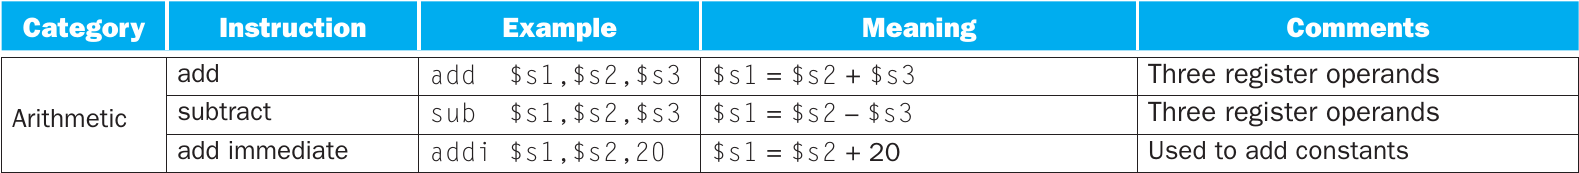
\includegraphics[width=\textwidth, height=0.2\textheight]{docs/images/operations-1}
\end{center}
\end{figure}
\end{frame}

\begin{frame}{Example - Compiling a C Assignment Using Registers}
\begin{flushleft}
It is the compiler’s job to associate program variables with registers. 

Take, for instance, the assignment statement from our earlier example:

\hspace{8mm}\texttt{f = (g + h) – (i + j);}

The variables \texttt{f}, \texttt{g}, \texttt{h}, \texttt{i}, and \texttt{j} are assigned to the registers \texttt{\$s0}, \texttt{\$s1}, \texttt{\$s2}, \texttt{\$s3},
and \texttt{\$s4}, respectively. 

What is the compiled MIPS code?
\end{flushleft}
\end{frame}

\begin{frame}[fragile]{Answer}
\begin{itemize}
\item[-]
\texttt{add \$t0, \$s1, \$s2  \# register \$t0 contains g + h}

\item[-]
\texttt{add \$t1, \$s3, \$s4  \# register \$t1 contains i + j}

\item[-]
\texttt{sub \$s0, \$t0, \$t1  \# f gets \$t0 – \$t1, which is (g + h) – (i + j)}
\end{itemize}
\end{frame}

\begin{frame}{Operations of the Computer Hardware (Cont'd)}
\begin{table}[H]
\begin{adjustbox}{width=\textwidth}
\begin{tabular}{|c|c|c|c|}
\hline
load word & \texttt{lw \$s1, 20(\$s2)} & \texttt{\$s1 = Memory[\$s2 + 20]} & Word from memory to register \\
\hline
store word & \texttt{sw \$s1, 20(\$s2)} & \texttt{Memory[\$s2 + 20] = \$s1} & Word from register to memory \\
\hline
load byte & \texttt{lb \$s1, 20(\$s2)} & \texttt{\$s1 = Memory[\$s2 + 20]} & Byte from memory to register \\
\hline
load byte unsigned & \texttt{lbu \$s1, 20(\$s2)} & \texttt{\$s1 = Memory[\$s2 + 20]} & Byte from memory to register \\
\hline
store byte & \texttt{sb \$s1, 20(\$s2)} & \texttt{Memory[\$s2 + 20] = \$s1} & Byte from register to memory \\
\hline
load upper immed & \texttt{lui \$s1, 20} & \texttt{\$s1 = 20 * $2^{16}$} & Loads constant in upper 16 bits \\
\hline
\end{tabular}
\end{adjustbox}
\caption{Data Transfer Instructions in MIPS}
\end{table}
\end{frame}

\begin{frame}{Example - Compiling Using Load and Store}
\begin{flushleft}
Assume variable \texttt{h} is associated with register \texttt{\$s2} and the base address of the array \texttt{A} is in \texttt{\$s3}. 

What is the MIPS assembly code for the C assignment state­
ment below?

\hspace{8mm}\texttt{A[12] = h + A[8];}
\end{flushleft}
\end{frame}

\begin{frame}{Answer}
\begin{itemize}
\item[-]
\texttt{lw \$t0, 32(\$s3) \# Temporary reg \$t0 gets A[8]}

\item[-]
\texttt{add \$t0, \$s2, \$t0  \# Temporary reg \$t0 gets h + A[8]}

\item[-]
\texttt{sw \$t0, 48(\$s3)  \# Stores h + A[8] back into A[12]}
\end{itemize}    
\end{frame}

\begin{frame}{Operations of the Computer Hardware (Cont'd)}
\begin{figure}\caption{Logical Instructions in MIPS}
\begin{center}
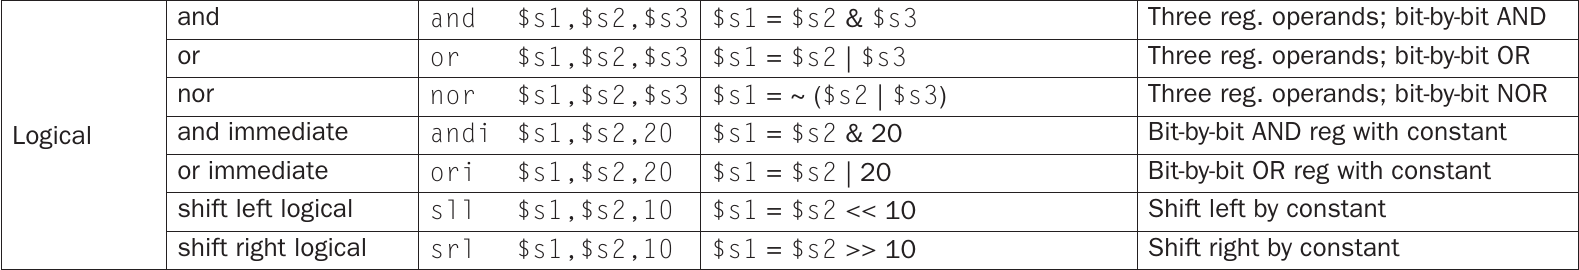
\includegraphics[width=\textwidth, height=0.4\textheight]{docs/images/operations-3}
\end{center}
\end{figure}
\end{frame}

\begin{frame}{Operations of the Computer Hardware (Cont'd)}
\begin{figure}\caption{Conditional Branch Instructions in MIPS}
\begin{center}
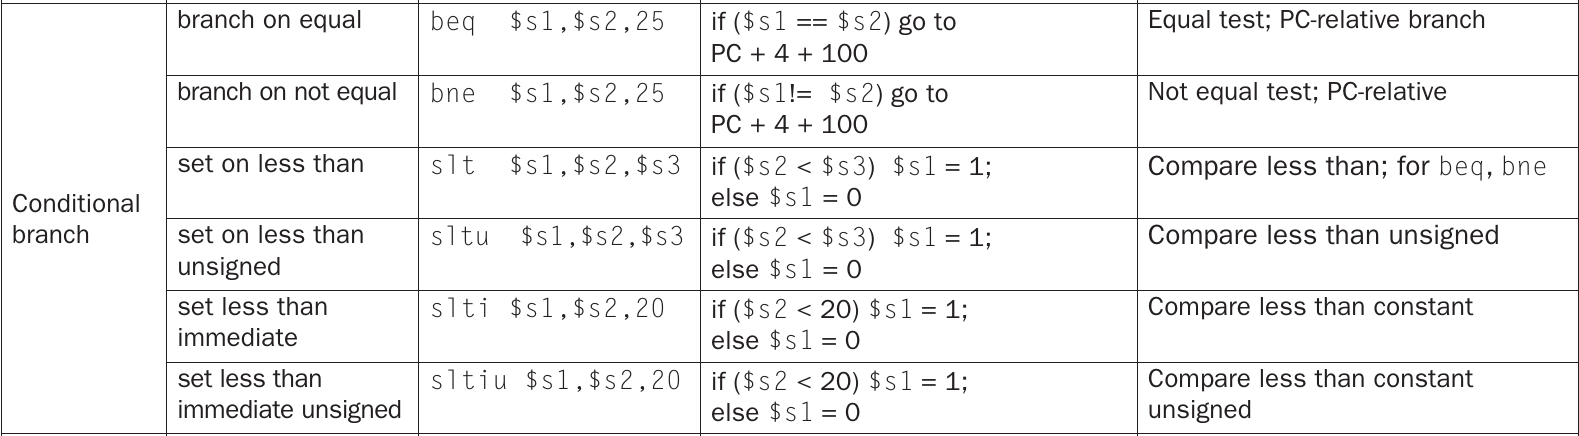
\includegraphics[width=\textwidth, height=0.5\textheight]{docs/images/operations-4}
\end{center}
\end{figure}
\end{frame}

\begin{frame}{Operations of the Computer Hardware (Cont'd)}
\begin{figure}\caption{Unconditional Jump Instructions in MIPS}
\begin{center}
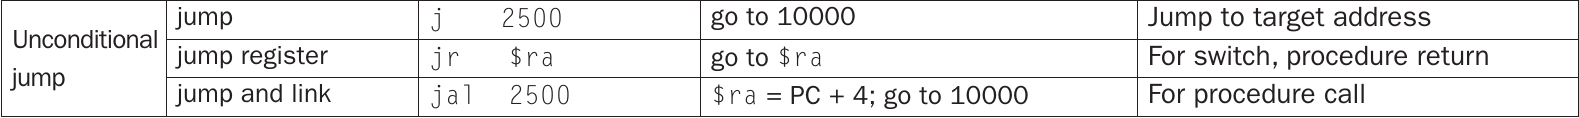
\includegraphics[width=\textwidth, height=0.17\textheight]{docs/images/operations-5  }
\end{center}
\end{figure}
\end{frame}

\section{Representing Instructions}
\begin{frame}{Instructions Big Picture}
\begin{table}[H]
\begin{adjustbox}{width=\textwidth}
\begin{tabular}{|c|c|c|c|c|c|c|c|c|}
\hline
Name & Format & \multicolumn{6}{|c|}{Example} & Comments \\
\hline
\hline
Field Size && 6 bit & 5 bit & 5 bit & 5 bit & 5 bit & 6 bit & All MIPS instructions are 32 bits long \\
\hline
R-format & R & op & rs & rt & rd & shamt & funct & Arithmetic instruction format \\
\hline
\texttt{add} & R & 0 & 18 & 19 & 17 & 0 & 32 & add \texttt{\$s1,\$s2,\$s3} \\
\hline
I-format & I & op & rs & rt & \multicolumn{3}{|c|}{address} & Data transfer format\\
\hline
\texttt{lw} & I & 35 & 18 & 17 & \multicolumn{3}{|c|}{100} & lw \texttt{\$s1,100(\$s2)} \\
\hline
J-format & J & op & \multicolumn{5}{|c|}{address} & Unconditional Branch \\
\hline
\texttt{j} & J & 8 & \multicolumn{5}{|c|}{300} & jump to address \\
\hline
\end{tabular}
\end{adjustbox}
\end{table}
\end{frame}

\section{Logical Operations}
\begin{frame}{Logical Operations Big Picture}
\begin{figure}
\begin{center}
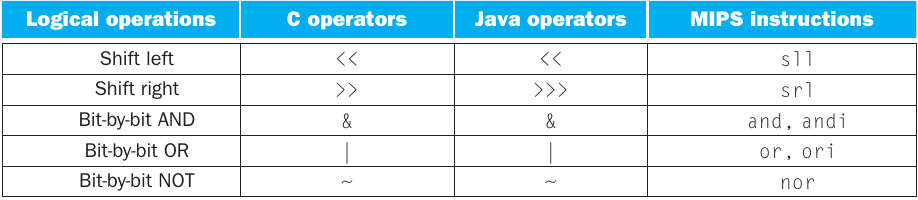
\includegraphics[width=\textwidth, height=0.4\textheight]{docs/images/logical}
\end{center}
\end{figure}
\end{frame}

\section{Instuctions for Making Decisions}
\begin{frame}{Instructions for Making Decisions}
\begin{itemize}
\item[-]
\texttt{beq register1, register2, L1}

This instruction means go to the statement labeled \texttt{L1} if the value in \texttt{register1}
equals the value in \texttt{register2}.

The mnemonic beq stands for \textit{branch if equal}.

\vspace{5mm}
\item[-]
\texttt{bne register1, register2, L1}

It means go to the statement labeled \texttt{L1} if the value in \texttt{register1} does not equal
the value in \texttt{register2}.

The mnemonic \texttt{bne} stands for \textit{branch if not equal}.
\end{itemize}
\end{frame}

\begin{frame}[fragile]{Example - Compiling \textit{if-then-else} into Conditional Branches}
\begin{flushleft}
In the following code segment, \texttt{f}, \texttt{g}, \texttt{h}, \texttt{i}, and \texttt{j} are variables. 

If the five variables, \texttt{f} through \texttt{j}, correspond to the five registers \texttt{\$s0} through \texttt{\$s4}, what is the
compiled MIPS code for this C if statement?

\begin{lstlisting}[language=python, keywordstyle=\color{purple}\textbf]
if i == j:
    f = g + h
else:
    f = g – h
\end{lstlisting}
\end{flushleft}
\end{frame}

\begin{frame}[fragile]{Answer}
\begin{lstlisting}[keywords={bne, add, j, sub}, keywordstyle=\color{purple}\textbf]
bne $s3, $s4, Else       # go to Else if i != j
add $s0, $s1, $s2        # f = g + h (skipped if i != j)
j   Exit                 # go to Exit
Else: 
    sub $s0, $s1, $s2    # f = g – h (skipped if i = j)
Exit:
\end{lstlisting}    
\end{frame}

\begin{frame}[fragile]{Example - Compiling a \textit{while} Loop in C}
\begin{flushleft}
Here is a traditional loop in C:
\begin{lstlisting}[language=c, keywordstyle=\color{purple}\textbf]
while (save[i] == k){
    i += 1;
}
\end{lstlisting}

Assume that \texttt{i} and \texttt{k} correspond to registers \texttt{\$s3} and \texttt{\$s5} and the base of the
array \texttt{save} is in \texttt{\$s6}.

What is the MIPS assembly code corresponding to this
C segment?
\end{flushleft}
\end{frame}

\begin{frame}[fragile]{Answer}
\begin{lstlisting}[keywords={sll, add, lw, bne, addi, j}, keywordstyle=\color{purple}\textbf]
Loop:   sll     $t1,$s3,2       # Temp reg $t1 = i * 4
        add     $t1,$t1,$s6     # $t1 = address of save[i]
        lw      $t0,0($t1)      # Temp reg $t0 = save[i]
        bne     $t0,$s5, Exit   # go to Exit if save[i] != k
        addi    $s3,$s3,1       # i = i + 1
        j       Loop            # go to Loop
Exit:
\end{lstlisting}
\end{frame}

\section{Suporting Precedures in Computer Hardware}
\begin{frame}{Six Steps}
\begin{enumerate}
\item Put parameters in a place where the procedure can access them.
\item Transfer control to the procedure.
\item Acquire the storage resources needed for the procedure. 
\item Perform the desired task.
\item Put the result value in a place where the calling program can access it. 
\item Return control to the point of origin, since a procedure can be called from several points in a program.
\end{enumerate}
\end{frame}

\begin{frame}{Provided Registers}
\begin{flushleft}
MIPS software follows the following convention for procedure calling in allocating its 32 registers
\end{flushleft}

\begin{itemize}
\item[-]
\texttt{\$a0-\$a3}: four argument registers in which to pass parameters
\item[-] \texttt{\$v0-\$v1}: two value registers in which to return values
\item[-] \texttt{\$ra}: one return address register to return to the point of origin    
\end{itemize}
\end{frame}

\begin{frame}{Provided Registers (Cont'd)}
\begin{itemize}
\item[-] In addition to allocating these registers, MIPS assembly language includes an instruction just for the procedures: 

\item[-]\textit{It jumps to an address and simultaneously saves the address of the following instruction in register \texttt{\$ra}.} 

\item[-]The \textit{jump-and-link} instruction (\texttt{jal}) is simply written:

\item[-] \texttt{jal ProcedureAddress}
\end{itemize}
\end{frame}

\begin{frame}{Provided Registers (Cont'd)}
\begin{itemize}
\item[-] 
The \textit{link} portion of the name means that an address or link is formed that points to
the calling site to allow the procedure to return to the proper address. This ``link",
stored in register \$ra (register 31), is called the return address. 

\item[-] The return address
is needed because the same procedure could be called from several parts of the
program.

\item[-]To support such situations, computers like MIPS use jump register instruction
(\texttt{jr}), introduced above to help with case statements, meaning an unconditional
jump to the address specified in a register:

\item[-] \texttt{jr \$ra}
\end{itemize}
\end{frame}

\begin{frame}[fragile]{Example - Compiling a C Procedure That Doesn’t Call Another Procedure}
\begin{lstlisting}[language=c, keywordstyle=\color{purple}\textbf]
int leaf_example (int g, int h, int i, int j)
{
    int f;
    f = (g + h) – (i + j);
    return f;
}
\end{lstlisting}
\end{frame}

\begin{frame}[fragile]{Answer}
\begin{lstlisting}[keywordstyle=\color{purple}\textbf, keywords={addi, sw, add, sub, lw, jr}, , numbers=none]
leaf_example:
    addi $sp, $sp, –12   # adjust stack to make room for 3 items
    sw   $t1, 8($sp)     # save register $t1 for use afterwards
    sw   $t0, 4($sp)     # save register $t0 for use afterwards
    sw   $s0, 0($sp)     # save register $s0 for use afterwards
    
    add  $t0, $a0, $a1   # register $t0 contains g + h
    add  $t1, $a2, $a3   # register $t1 contains i + j
    sub  $s0, $t0, $t1   # f = $t0 – $t1, which is (g + h)–(i + j)
    
    add  $v0, $s0, $zero # returns f ($v0 = $s0 + 0)    
\end{lstlisting}
\end{frame}

\begin{frame}[fragile]{Answer (Cont'd)}
\begin{lstlisting}[keywordstyle=\color{purple}\textbf, keywords={addi, sw, add, sub, lw, jr}, numbers=none]
    lw   $s0, 0($sp)     # restore register $s0 for caller
    lw   $t0, 4($sp)     # restore register $t0 for caller
    lw   $t1, 8($sp)     # restore register $t1 for caller
    addi $sp, $sp, 12    # adjust stack to delete 3 items

    jr   $ra             # jump back to calling routine 
\end{lstlisting}
\end{frame}

\begin{frame}[fragile]{Example - Compiling a Recursive C Procedure, Showing Nested Procedure
        Linking}
\begin{lstlisting}[keywordstyle=\color{purple}\textbf, language=c]
int fact (int n)
{
    if (n < 1) {
        return 1;
    }
    else {
        return (n * fact(n – 1));
    }
}
\end{lstlisting}
\end{frame}

\begin{frame}[fragile]{Answer}
\begin{lstlisting}[keywordstyle=\color{purple}\textbf, keywords={addi, sw, slti, beq, jr}, , numbers=none]
fact:
    addi $sp, $sp, –8   # adjust stack for 2 items
    sw   $ra, 4($sp)    # save the return address
    sw   $a0, 0($sp)    # save the argument n
    
    slti $t0, $a0, 1    # test for n < 1
    beq  $t0, $zero, L1 # if n >= 1, go to L1
    
    addi $v0, $zero, 1  # return 1
    addi $sp, $sp, 8    # pop 2 items off stack
    jr $ra              # return to caller
\end{lstlisting}
\end{frame}

\begin{frame}[fragile]{Answer (Cont'd)}
\begin{lstlisting}[keywordstyle=\color{purple}\textbf, keywords={addi, jal, lw, mul, jr}, numbers=none]
L1: 
    addi $a0, $a0, –1  # n >= 1: argument gets (n – 1)
    jal fact           # call fact with (n – 1)

    lw $a0, 0($sp)     # return from jal: restore argument n
    lw $ra, 4($sp)     # restore the return address
    addi $sp, $sp, 8   # adjust stack pointer to pop 2 items
    
    mul $v0, $a0, $v0  # return n * fact (n – 1)

    jr $ra             # return to the caller
\end{lstlisting}
\end{frame}

\section{MIPS Addressing for 32-Bit Immediates and Addresses}
\begin{frame}{Example - Loading a 32-Bit Constant}
\begin{flushleft}
What is the MIPS assembly code to load this 32-bit constant into register \texttt{\$s0}?

\hspace{8mm}\texttt{0000 0000 0011 1101 0000 1001 0000 0000}
\end{flushleft}
\end{frame}

\begin{frame}[fragile]{Answer}
\begin{lstlisting}[keywordstyle=\color{purple}\textbf, keywords={lui, ori}]
lui $s0, 61  # 61 decimal = 0000 0000 0011 1101 binary

# value of $s0 
# 0000 0000 0011 1101 0000 0000 0000 0000

ori $s0, $s0, 2304 # 2304 decimal = 0000 1001 0000 0000

# final value of #s0
# 0000 0000 0011 1101 0000 1001 0000 0000
\end{lstlisting}
\end{frame}

\begin{frame}{Illustration of the five MIPS addressing modes}
\begin{itemize}
\item[-]  Immediate addressing

where the operand is a constant within the instruc-
tion itself 
\end{itemize}
\begin{figure}
\begin{center}
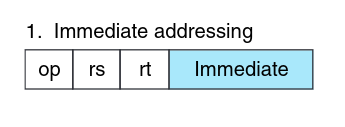
\includegraphics[width=0.6\textwidth, height=0.4\textheight]{docs/images/addr-1}
\end{center}
\end{figure}
\end{frame}

\begin{frame}{Illustration of the five MIPS addressing modes (Cont'd)}
\begin{itemize}
\item[-] Register addressing

where the operand is a register
\end{itemize}
    
\begin{figure}
\begin{center}
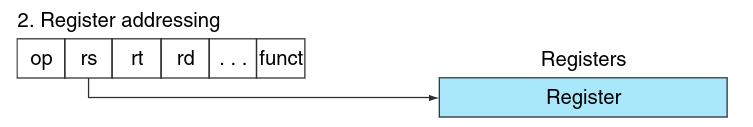
\includegraphics[width=0.8\textwidth, height=0.25\textheight]{docs/images/addr-2}
\end{center}
\end{figure}
\end{frame}


\begin{frame}{Illustration of the five MIPS addressing modes (Cont'd)}
\begin{itemize}
\item[-] Base or displacement addressing

where the operand is at the memory location whose address is the sum of a register and a constant in the instruction
\end{itemize}

\begin{figure}
\begin{center}
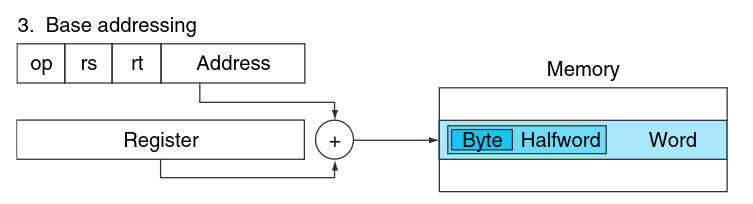
\includegraphics[width=0.8\textwidth, height=0.4\textheight]{docs/images/addr-3}
\end{center}
\end{figure}
\end{frame}

\begin{frame}{Illustration of the five MIPS addressing modes (Cont'd)}
    
\begin{itemize}
\item[-] PC-relative addressing

where the branch address is the sum of the PC and a
constant in the instruction
\end{itemize}

\begin{figure}
\begin{center}
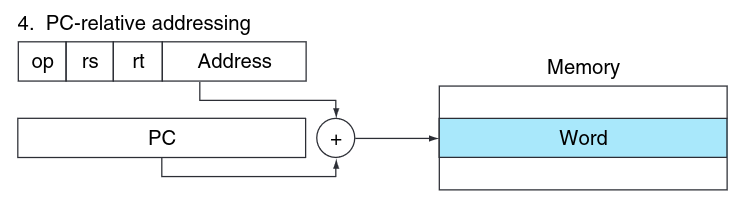
\includegraphics[width=0.8\textwidth, height=0.45\textheight]{docs/images/addr-4}
\end{center}
\end{figure}
\end{frame}
\begin{frame}{Illustration of the five MIPS addressing modes (Cont'd)}

\begin{itemize}
\item[-] Pseudodirect addressing

where the jump address is the 26 bits of the instruction concatenated with the upper bits of the PC
\end{itemize}

\begin{figure}
\begin{center}
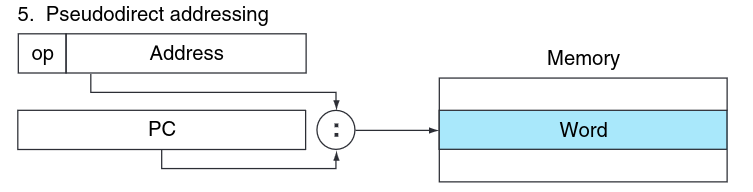
\includegraphics[width=0.8\textwidth, height=0.4\textheight]{docs/images/addr-5}
\end{center}
\end{figure}
\end{frame}

\section{A C Sort Example to Put It All Together}
\begin{frame}[fragile]{A C procedure that swaps two locations in memory}
\begin{lstlisting}[language=c, keywordstyle=\color{purple}\textbf]
void swap(int v[], int k)
{
    int temp;
    temp = v[k];
    v[k] = v[k+1];
    v[k+1] = temp;
}
\end{lstlisting}
\end{frame}

\begin{frame}{What to do?}
\begin{enumerate}
\item
Allocate registers to program variables.

\item
Produce code for the body of the procedure.

\item
Preserve registers across the procedure invocation.
\end{enumerate}
\end{frame}

\begin{frame}{Register Allocation for \texttt{swap}}
\begin{itemize}
\item[-] Since swap has just two parameters, \texttt{v} and
\texttt{k}, they will be found in registers \texttt{\$a0} and \texttt{\$a1}. 

\item[-]The only other variable is \texttt{temp},
which we associate with register \texttt{\$t0}
\end{itemize}
\end{frame}

\begin{frame}[fragile]{Code for the Body of the Procedure \texttt{swap}}
\begin{lstlisting}[keywordstyle=\color{purple}\textbf, keywords={sll, add, lw, jr, sw}]
swap: 
    sll $t1, $a1, 2    # reg $t1 = k * 4
    add $t1, $a0, $t1  # reg $t1 = v + (k * 4)
                       # reg $t1 has the address of v[k]
    
    lw $t0, 0($t1)     # reg $t0 (temp) = v[k]
    lw $t2, 4($t1)     # reg $t2 = v[k + 1]
                       # refers to next element of v
    
    sw $t2, 0($t1)     # v[k] = reg $t2
    sw $t0, 4($t1)     # v[k+1] = reg $t0 (temp)
    
    jr $ra             # return to calling routine
\end{lstlisting}
\end{frame}

\begin{frame}[fragile]{A C procedure that performs a sort on the array \texttt{v}}
\begin{lstlisting}[language=c, keywordstyle=\color{purple}\textbf]
void sort (int v[], int n)
{
    int i, j;
    for (i = 0; i < n; i += 1) {
        for (
            j = i – 1;
            j >= 0 && v[j] > v[j + 1];
            j = 1
        ) {
            swap(v,j);
        }
    }
}
\end{lstlisting}
\end{frame}

\begin{frame}{Register Allocation for \texttt{sort}}
\begin{itemize}
\item[-]The two parameters of the procedure \texttt{sort}, \texttt{v} and \texttt{n}, are in the parameter registers
\texttt{\$a0} and \texttt{\$a1}, 

\item[-] and we assign register \texttt{\$s0} to \texttt{i} and register \texttt{\$s1} to \texttt{j}
\end{itemize}
\end{frame}

\begin{frame}[fragile]{Code for the Body of the Procedure \texttt{sort}}
\begin{flushleft}
Saving registers
\begin{lstlisting}[keywordstyle=\color{purple}\textbf, keywords={addi, sw}, numbers=none]
sort: 
    addi $sp, $sp, –20  # make room on stack for 5 registers
    sw   $ra, 16($sp)   # save $ra on stack
    sw   $s3, 12($sp)   # save $s3 on stack
    sw   $s2, 8($sp)    # save $s2 on stack
    sw   $s1, 4($sp)    # save $s1 on stack
    sw   $s0, 0($sp)    # save $s0 on stack
    ...
\end{lstlisting}
\end{flushleft}
\end{frame}

\begin{frame}[fragile]{Code for the Body of the Procedure \texttt{sort} (Cont'd)}
\begin{flushleft}
Move parameters 
\begin{lstlisting}[keywordstyle=\color{purple}\textbf, keywords={move}, numbers=none]
    ...
    move $s2, $a0      # copy parameter $a0 into $s2 (save $a0)
    move $s3, $a1      # copy parameter $a1 into $s3 (save $a1)
    ...
\end{lstlisting}
\end{flushleft}
\end{frame}

\begin{frame}[fragile]{Code for the Body of the Procedure \texttt{sort} (Cont'd)}
\begin{flushleft}
Outer loop
\begin{lstlisting}[keywordstyle=\color{purple}\textbf, keywords={move, slt, beq}, numbers=none]
...
    move $s0, $zero         # i = 0
for1tst: 
    slt  $t0, $s0, $s3      # reg $t0 = 0 if $s0 Š $s3 (i Š n)
    beq  $t0, $zero, exit1  # go to exit1 if $s0 Š $s3 (i Š n)
...
\end{lstlisting}
\end{flushleft}
\end{frame}

\begin{frame}[fragile]{Code for the Body of the Procedure \texttt{sort} (Cont'd)}
\begin{flushleft}
Inner loop
\begin{lstlisting}[keywordstyle=\color{purple}\textbf, keywords={addi, slti, bne, add, sll, lw, slt, beq}, numbers=none]
...
    addi $s1, $s0, –1       # j = i – 1
for2tst: 
    slti $t0, $s1, 0        # reg $t0 = 1 if $s1 < 0 (j < 0)
    bne  $t0, $zero, exit2  # go to exit2 if $s1 < 0 (j < 0)
    sll  $t1, $s1, 2        # reg $t1 = j * 4
    add  $t2, $s2, $t1      # reg $t2 = v + (j * 4)
    lw   $t3, 0($t2)        # reg $t3 = v[j]
    lw   $t4, 4($t2)        # reg $t4 = v[j + 1]
    slt  $t0, $t4, $t3      # reg $t0 = 0 if $t4 Š $t3
    beq  $t0, $zero, exit2  # go to exit2 if $t4 Š $t3
...
\end{lstlisting}
\end{flushleft}
\end{frame}

\begin{frame}[fragile]{Code for the Body of the Procedure \texttt{sort} (Cont'd)}
    \begin{flushleft}
Pass parameters and call \texttt{swap}
\begin{lstlisting}[keywordstyle=\color{purple}\textbf, keywords={move, jal}, numbers=none]
...
    move $a0, $s2  # 1st parameter of swap is v (old $a0)
    move $a1, $s1  # 2nd parameter of swap is j
    jal  swap       # swap
...
\end{lstlisting}
\end{flushleft}
\end{frame}

\begin{frame}[fragile]{Code for the Body of the Procedure \texttt{sort} (Cont'd)}
\begin{flushleft}
Inner loop
\begin{lstlisting}[keywordstyle=\color{purple}\textbf, keywords={addi, j}, numbers=none]
...
    addi $s1, $s1, –1  # j –= 1
    j    for2tst       # jump to test of inner loop
...
\end{lstlisting}
\end{flushleft}
\end{frame}

\begin{frame}[fragile]{Code for the Body of the Procedure \texttt{sort} (Cont'd)}
\begin{flushleft}
Outer loop
\begin{lstlisting}[keywordstyle=\color{purple}\textbf, keywords={addi, j}, numbers=none]
...
exit2:
    addi $s0, $s0, 1  # i += 1
    j    for1tst      # jump to test of outer loop
...
\end{lstlisting}
\end{flushleft}
\end{frame}

\begin{frame}[fragile]{Code for the Body of the Procedure \texttt{sort} (Cont'd)}
\begin{flushleft}
Restoring Registers
\begin{lstlisting}[keywordstyle=\color{purple}\textbf, keywords={lw, addi}, numbers=none]
...
exit1: 
    lw   $s0, 0($sp)  # restore $s0 from stack
    lw   $s1, 4($sp)  # restore $s1 from stack
    lw   $s2, 8($sp)  # restore $s2 from stack
    lw   $s3,12($sp)  # restore $s3 from stack
    lw   $ra,16($sp)  # restore $ra from stack
    addi $sp,$sp, 20  # restore stack pointer
...
\end{lstlisting}
\end{flushleft}
\end{frame}

\begin{frame}[fragile]{Code for the Body of the Procedure \texttt{sort} (Cont'd)}
\begin{flushleft}
Procedure return
\begin{lstlisting}[keywordstyle=\color{purple}\textbf, keywords={jr}, numbers=none]
...
jr $ra # return to calling routine
\end{lstlisting}
\end{flushleft}
\end{frame}
